\documentclass[12pt]{article}
\usepackage{fullpage}
\usepackage{amsmath}
\usepackage{amssymb}
\usepackage{amsthm}
\usepackage{graphicx}
\usepackage{subfigure}
\usepackage{ dsfont }
\usepackage{ mathrsfs }
\usepackage{ mathtools }
\usepackage{hyperref}
%\usepackage{cite}
\usepackage[round]{natbib}
\usepackage{caption}
\usepackage{array}
\usepackage{titling}

%% --------------------- option1 to put Julia code
%% Julia definition (c) 2014 Jubobs
%%
\usepackage{listings}
\usepackage{xcolor}
\definecolor{light-gray}{gray}{0.95}

\lstdefinelanguage{Julia}%
  {morekeywords={abstract,break,case,catch,const,continue,do,else,elseif,%
      end,export,false,for,function,immutable,import,importall,if,in,%
      macro,module,otherwise,quote,return,switch,true,try,type,typealias,%
      using,while,include},%
   sensitive=true,%
%   alsoother={$},%
   morecomment=[l]\#,%
   morecomment=[n]{\#=}{=\#},%
   morestring=[s]{"}{"},%
   morestring=[m]{'}{'},%
}[keywords,comments,strings]%

\lstset{%
    language         = Julia,
    basicstyle       = \ttfamily,
    keywordstyle     = \bfseries\color{blue},
    stringstyle      = \color{magenta},
    commentstyle     = \color{ForestGreen},
    showstringspaces = false,
    backgroundcolor=\color{light-gray},
}

%------------------------------option2 to put Julia code
%%%%% https://gist.github.com/chi-feng/6589066

% \usepackage{inconsolata} % very nice fixed-width font included with texlive-full
% \usepackage[usenames,dvipsnames]{color} % more flexible names for syntax highlighting colors
% \usepackage{listings}

% \lstset{
% basicstyle=\ttfamily,
% columns=fullflexible, % make sure to use fixed-width font, CM typewriter is NOT fixed width
% numbers=left,
% numberstyle=\small\ttfamily\color{Gray},
% stepnumber=1,
% numbersep=10pt,
% numberfirstline=true,
% numberblanklines=true,
% tabsize=4,
% lineskip=-1.5pt,
% extendedchars=true,
% breaklines=true,
% keywordstyle=\color{Blue}\bfseries,
% identifierstyle=, % using emph or index keywords
% commentstyle=\sffamily\color{OliveGreen},
% stringstyle=\color{Maroon},
% showstringspaces=false,
% showtabs=false,
% upquote=false,
% texcl=true % interpet comments as LaTeX
% }

% \lstdefinelanguage{julia}
% {
%   keywordsprefix=\@,
%   morekeywords={
%     exit,whos,edit,load,is,isa,isequal,typeof,tuple,ntuple,uid,hash,finalizer,convert,promote,
%     subtype,typemin,typemax,realmin,realmax,sizeof,eps,promote_type,method_exists,applicable,
%     invoke,dlopen,dlsym,system,error,throw,assert,new,Inf,Nan,pi,im,begin,while,for,in,return,
%     break,continue,macro,quote,let,if,elseif,else,try,catch,end,bitstype,ccall,do,using,module,
%     import,export,importall,baremodule,immutable,local,global,const,Bool,Int,Int8,Int16,Int32,
%     Int64,Uint,Uint8,Uint16,Uint32,Uint64,Float32,Float64,Complex64,Complex128,Any,Nothing,None,
%     function,type,typealias,abstract
%   },
%   sensitive=true,
%   morecomment=[l]{\#},
%   morestring=[b]',
%   morestring=[b]"
% }

\bibliographystyle{mbe} %needs mbe.bst

\newcommand{\falta}[1]{\textcolor{red}{#1}}

\pretitle{%
  \begin{center}
  \LARGE
  \includegraphics[width=6cm,height=2cm]{figures/SNaQ-final-green.pdf}\\[\bigskipamount]
}
\posttitle{\end{center}}

\title{\texttt{PhyloNetworks} Documentation\\
 \large Version 0.0.2}
\author{Claudia Sol\'{i}s-Lemus, C\'{e}cile An\'{e} and John Spaw}
%\date{}

\begin{document}
% http://tex.stackexchange.com/questions/212793/how-can-i-typeset-julia-code-with-the-listings-package
% to put julia code in latex

\maketitle

\section{Introduction}
\texttt{PhyloNetworks} is a \texttt{Julia} package with several
functions for phylogenetic networks, among which we can highlight
reading from and writing in parenthetical format, re-rooting and
plotting.  The main estimation function in \texttt{PhyloNetworks} is
the method \texttt{SNaQ} (Species Networks applying Quartets): a
statistical method to infer a phylogenetic network from input gene
trees \citep{Solis-Lemus2015}.

\paragraph{Assumption on the phylogenetic network.} For now,
\texttt{SNaQ} assume that the hybridization cycles do not intersect,
and these networks are called \textit{level-1 networks}
\citep{Huson2010}. See the appendix for more details on the definition
of phylogenetic networks used here.  This restriction (and others
mentioned in the appendix) is enforced in the optimization, but not in
the read/write/plot/root functions. However, the only rule strictly
enforced for all functions is that a hybrid node cannot have more than
two hybrid edges pointing to it.
% This is a restriction that we hope to
% eliminate in the future.

\paragraph{Why Julia?} Julia is a high-level and interactive
programming language (like R or Matlab), but it is also
high-performance (like C). So, it is fast. However, there is a minor
drawback in Julia versions 0.3 (or lower): Julia code is just-in-time
compiled which means that the first time you run a function, it will
take a lot of time because it will compile it. It is important to keep
this in mind as we use Julia, because the next calls for a function
will be much much faster. So, please be patient! Trying out small toy
examples for the first calls of functions is always a good idea.


\section{Setup}
\subsection{Installation of \texttt{Julia}}
To install \texttt{Julia} go to \url{http://julialang.org/downloads/}.\\
\texttt{PhyloNetworks} was developed under \texttt{Julia}
version 0.3.5, but the package is fully migrated to version 0.4.
Issues may arise by using a version of Julia lower than 0.4.

\subsection{Installation of \texttt{PhyloNetworks}}
To install the package,
open
\texttt{Julia} and type:
\begin{lstlisting}
Pkg.clone("https://github.com/crsl4/PhyloNetworks.git")
Pkg.build("PhyloNetworks")
\end{lstlisting}

The \texttt{PhyloNetworks} package has the following dependencies, but everything is installed when
\texttt{PhyloNetworks} is added.
\begin{itemize}
\item \texttt{GraphViz} (version 0.0.3)
\item \texttt{NLopt} (version 0.2.0)
\end{itemize}
The version in parenthesis correspond to the ones used when
implementing \texttt{PhyloNetworks}.
To test that you installed correctly the \texttt{PhyloNetworks} package, try the following example:

\subsubsection{Example to test correct \texttt{PhyloNetworks} installation}
Open \texttt{Julia} and type
\begin{lstlisting}
Pkg.test("PhyloNetworks")
\end{lstlisting}
This will take a couple of
minutes as the package needs to compile all the functions. If the
installation was successful, you will see a message at the end:
\textcolor{green}{\textbf{Tests passed}}. Otherwise, an error will be thrown.

\section{Usage of PhyloNetworks}
Before each session, need to type in \texttt{Julia}:

\begin{lstlisting}
using PhyloNetworks
\end{lstlisting}

This will take a couple of minutes as it needs to precompile the
functions.  The first run of a function in \texttt{Julia} will also
compile, so it will be slower than any subsequent runs.

\subsection{Basic Julia commands}
Pressing \textbf{?} inside Julia followed by a command will prompt the
documentation of such command.
\begin{lstlisting}
? typeof
a=4
typeof(a)
whos()
\end{lstlisting}


\section{Update of PhyloNetworks}
It is important to regularly update the version of the Julia packages:

\begin{lstlisting}
Pkg.update()
\end{lstlisting}

This will take a couple of minutes as it needs to precompile the
functions in every package. This is particulary important for the
package \texttt{PhyloNetworks} since it is a new package under constant
development.

% \paragraph{WARNING:} There is a known bug for Mac users where the \texttt{Pkg.update} function does not update to the latest version. We recommend Mac users to do the following through the terminal:\\
% \texttt{
%   cd HOME/.julia/v0.3/PhyloNetworks/ \\
%   git pull } \\where HOME is replaced by your home directory and v0.3
% could be replaced by v0.4 if you have version 0.4 of Julia.

\section{Description of the main types}
\label{types}

\begin{itemize}
\item{\textbf{HybridNetwork:} Explicit phylogenetic network or
    phylogenetic tree. The object can be rooted or unrooted (in the
    case of network, it would be semi-directed).It has the following
    main attributes:
\begin{itemize}
\item{numTaxa: number of taxa}
\item{numNodes: number of nodes}
\item{numEdges: number of edges}
\item{node: array of Nodes}
\item{edge: array of Edges}
\item{root: index in node for the root}
\item{loglik: -log pseudolik after SNaQ estimation}
\end{itemize}
}
\item{\textbf{DataCF:} Type that holds the input data, and it has the following
  attributes:
\begin{itemize}
\item{quartet: array of 4-taxon subsets (type \texttt{Quartet}) either read from a table of CF
  or chosen to be analyzed from a list of trees.}
\item{numQuartets: number of 4-taxon sets}
\item{tree: array of \texttt{HybridNetwork} if input data was a list of gene
    trees, empty if input data was table of CF}
\item{numTrees: number of trees in the case the DataCF was created
    from a list of gene trees (-1 otherwise)}
\item{repSpecies: taxon names that are repeated in the table of CF for
  the case of multiple alleles}
\end{itemize}
}
\item{\textbf{Quartet:} Object to hold the information of a given 4-taxon
    set. It has the following attributes:
\begin{itemize}
\item{number: 4-taxon sets are numbered}
\item{taxon: array of taxon names}
\item{obsCF: array of observed CF read from CF table or computed from
    input gene trees}
\item{logPseudolik: -log pseudolik}
\item{ngenes: number of genes used to compute the observed CF (-1 if
    observedCF read from CF table)}
\item{qnet: internal topological structure used in the
    optimization. This structure saves the expected CF after snaq
    estimation to emphasize that the expCF depend on a specific
    network, not on the data}
\end{itemize}
}
\end{itemize}

\section{Description of the main functions}
Functions in \texttt{Julia} that end with exclamation sign \textbf{!}
are modifying one (or all) of the arguments.
\paragraph{Important:} Functions in Julia have required arguments and
optional arguments. Required arguments \textbf{should not be
  named}. For example, you would call\\
\texttt{readTopology("(A,(B,(C,D)));")} not
\texttt{readTopology(net="(A,(B,(C,D)));")}. On the contrary, optional
arguments \textbf{have to be named.}
In the following descriptions, it is specified which arguments are
optional and which arguments are required. If there is only one
argument, it is required.

The description of the
functions in \texttt{PhyloNetworks} is next:
\begin{itemize}
\item \textbf{readTopology:} Read a tree or network from
  parenthetical format. Input can be a string or a name of a text file
  (this file should contain only one line with the tree in
  parenthetical format and end in ;, no quotes. To read more than one
  tree, see \texttt{readInputTrees} function
  instead). \texttt{readTopology} function returns a
  \texttt{HybridNetwork} object. This function allows for polytomies
  in tree nodes (tree node with more than two children) and allows for
  internal nodes with only two edges (one parent and one child).
%falta{(and other things not tested yet)}.
\\Usage:
\begin{lstlisting}
net=readTopology("file.txt");
net=readTopology("(A,(B,(C,D)));");
\end{lstlisting}

\item \textbf{readTopologyLevel1:} Same as \texttt{readTopology}, but
  enforces the restrictions that the network must be of
  level-1. \texttt{readTopology} should be used when you want more
  variety of topologies, but these topologies cannot be used directly
  as starting point in the \texttt{SNaQ} optimization method (which is
  taken care of automatically inside the optimization function). This
  function also returns a \texttt{HybridNetwork} object. \\
  Usage:
\begin{lstlisting}
 net=readTopologyLevel1("file.txt");
 net=readTopologyLevel1("(A,(B,(C,D)));");
\end{lstlisting}


\item \textbf{tipLabels:} Print the list of taxon names in the \texttt{HybridNetwork}
  object.
Usage:
\begin{lstlisting}
tipLabels(net)
\end{lstlisting}

\item \textbf{writeTopology:} Write the parenthetical format of a
  \texttt{HybridNetwork} object. The first argument is required and it
  is a \texttt{HybridNetwork} object. It has three optional arguments:
\begin{itemize}
\item{\textit{di=true}: to print in a format that Dendroscope can
    read, that is, without the $\gamma$ heritability values of hybrid
    edges (default false)}
\item{\textit{outgroup=taxon name}: to root by the outgroup before
    printing (default none). The outgroup has to be a single taxon. We will update to
  allow a clade in the future.}
\item{\textit{names=true}: to print the taxon names in the leaves as opposed to
  the node numbers (default true).}
\end{itemize}
Usage:
\begin{lstlisting}
writeTopology(net)
writeTopology(net,di=true)
\end{lstlisting}

\item \textbf{root!:} Re-root a network at a node or outgroup (single
  taxon). When a node number is used as parameter, \textit{resolve}
  argument is required. If true, a branch with zero length is
  added. The node numbers can be known with \texttt{printEdges,
    printNodes} functions described below or with the plot function
  described in section \ref{sectPlot}. All arguments are required.
  Usage:
\begin{lstlisting}
root!(net,nodeNumber,resolve)
root!(net,outgroup)
\end{lstlisting}

\item \textbf{deleteLeaf!:} Delete a leaf from a
  \texttt{HybridNetwork} object. Both arguments are required.
Usage:
\begin{lstlisting}
deleteLeaf!(net,taxonName)
\end{lstlisting}


\item \textbf{printEdges:} Print out the information on
  all the edges in a
  \texttt{HybridNetwork} object. Not all information is useful for the
  user, but information like \textit{edge length} and \textit{gamma}
  are printed.
Usage:
\begin{lstlisting}
printEdges(net)
\end{lstlisting}


\item \textbf{printNodes:} Print out the information on
  all the nodes in a
  \texttt{HybridNetwork} object. Not all information is useful for the
  user, but information like \textit{node number}
  could be, in particular.
Usage:
\begin{lstlisting}
printNodes(net)
\end{lstlisting}

\end{itemize}

\section{\texttt{SNaQ}: estimation of phylogenetic networks}

\subsection{Reading in data}
\texttt{SNaQ} estimates a phylogenetic network with the statistical
methodology described in \citet{Solis-Lemus2015}. There are two possible
input data:
\begin{itemize}
\item{List of estimated gene trees: Estimated gene trees can be
    obtained from sequence data using RAxML \citep{raxmlv8} or
    MrBayes \citep{Huelsenbeck2001}. Trees need to be in parenthetical
    format. Other formats will be available in future versions of the
    package.}
\item{Table of estimated quartet concordance factors (CF): Estimated
    CF on 4-taxon sets which can be obtained from estimated gene trees
    with BUCKy \cite{Ane2007}. A useful pipelin from sequences to CF
    can be found in \url{https://github.com/nstenz/TICR}.}
\end{itemize}
The methodology also requires a starting topology for the search. This
can be read from parenthetical format.

\noindent Functions to read data into \texttt{Julia}:
\begin{itemize}
\item \textbf{readTrees2CF:} Read a text file with a list of trees in
  parenthetical format (one tree per line, but it can have extra lines
  like headline that the function will ignore. It will assume that any
  line starting with ``(`` is a tree). The function will calculate the
  observed CFs of 4-taxon subsets.  This function has the following
  optional arguments:
\begin{itemize}
\item{\textit{quartetfile} (default empty): the list of desired
    4-taxon subsets to analyze can be given in a text file. If no
    such file is specified, the function will take either all the
    possible 4-taxon subsets or a random sample based on the following
    options.}
\item{\textit{whichQ} (default ``all''): if set to \textit{``rand''},
    the 4-taxon subsets will be chosen at random. If
    \textit{quartetfile} was defined, then the random sample is taken
    from the 4-taxon subsets in that file. If not, then the sample is
    drawn from all the possible 4-taxon subsets for the taxa in the
    input trees ($n \choose 4$ where $n$ is the total number of tips
    in the trees). The number of subsets to be chosen is set by the
    argument \textit{numQ}. If no such number is defined, by default
    the function will set it as 10\% of the total number of possible
    4-taxon subsets. \textbf{Important:} If \textit{numQ} is
    specified, but \textit{whichQ} is not set to "rand", then
    \textit{numQ} will be ignored.}
\item{\textit{CFfile} (default ``tableCF.txt''): name of the file to
    save the observed CFs computed from the input trees}
\item{\textit{writetab} (default true): if set to false, then no table
  of observed CF is written.}
\item{\textit{writeFile} (default false): if set to true, then text
    files with the list of the sampled 4-taxon subsets are
    created. Keep in mind that these files can be very big depending
    on the number of taxa.}
\item{\textit{taxa} (default union of all taxa in the tree file): you
    can choose the set of taxa for the quartets with the argument
    (vector of string names for chosen taxa).}
\end{itemize}

WARNING: This function has not yet been tested with missing data. That
is, it has been tested in
examples where all the trees have the same taxa.\\
Usage:
\begin{lstlisting}
readTrees2CF(treefile, quartetfile=..., whichQ=..., numQ=...,
             writetab=..., CFfile=..., writeFile=...)
\end{lstlisting}

\item \textbf{readTableCF:} Read a table of observed CF. The first 7
  columns in table should be as in Table \ref{tableCF}, but the table
  can have more columns which are ignored. The required
  argument is the name of the table file, but it also has an optional
  argument \textit{sep} for the character that
  separates columns in the table file.\\
\begin{table}[h]
\centering
\begin{tabular}{c|c|c|c|c|c|c}
Taxon1 & Taxon2 &Taxon3 & Taxon4 & $CF12|34$ & $CF13|24$ &  $CF14|23$\\
\hline \\
 & & & & & &
\end{tabular}
\caption{Example of column format for the table of CFs to be used as
  input data}
\label{tableCF}
\end{table}

Usage:
\begin{lstlisting}
readTableCF(filename);
readTableCF(filename, sep=';');
\end{lstlisting}
WARNING: It is important to use single quotes: ' not double quotes "
when specifying the separator in the table.

Both functions \texttt{readTrees2CF} and \texttt{readTableCF} return a
data structure called \texttt{DataCF} described in \ref{types}

\item \textbf{readInputTrees:} Read a text file containing a list of trees
  in parenthetical format (one per line, ignores any line that does
  not start on ``(``) and
  returns a vector of trees. The output is a vector of
  \texttt{HybridNetwork} objects, one per line read.
  Usage:
\begin{lstlisting}
readInputTrees(filename)
\end{lstlisting}

\item \textbf{summarizeCFdata:} Take as input a data structure
  \texttt{DataCF} (from previous functions) and provides a descriptive
  information. By default, it prints the information on the screen,
  but it can be saved to a file. The option \textit{pc} is used only
  when CFs were computed from a collection of gene trees: the CFs of
  4-taxon subsets that were computed with fewer than proportion
  \textit{pc} gene trees are listed. The option \textit{pc} should be
  a number between 0 and 1, and the default value is 0.7. The required
  argument is \textit{d}, the optional
  arguments are \textit{filename,pc} (followed by = below).
  Usage:
\begin{lstlisting}
summarizeCFdata(d)
summarizeCFdata(d,filename=...)
summarizeCFdata(d,filename=...,pc=...)
\end{lstlisting}

% \item \textbf{readStartTop:} Read a tree in parenthetical format from
%   a text file and updates its branch lengths in coalescent units to
%   fit the CF data on the data structure \texttt{DataCF}.  For each
%   branch in the tree, the average CF is computed for all the 4-taxon
%   subtrees that contain that branch. The branch length is then set as
%   $-log(3/2(1-\overline{CF}))$. It is equivalent to run
%   \texttt{net=readTopologyLevel1(treefile)} first and then \texttt{updateBL!(net,d)}.\\
%   WARNING: updateBL only works for a tree topology, not proven for a
%   network yet. Both arguments are required. \textbf{Only branch
%     lengths that are missing in the topology are updated.}  Updating
%   the mising branch lengths is done automatically inside
%   \texttt{SNaQ}, so there is no need to do this step before running
%   the estimation procedure.  Usage:
% \begin{lstlisting}
% readStartTop(treefile, d)
% \end{lstlisting}

\end{itemize}

\subsubsection{Small example on reading data}
\label{readDataEx}
All the files for this section can be downloaded from the
\textit{examples} folder in github repository. They need to be copied
in the working directory.  Suppose that the list of gene trees is
stored in file \textit{treefile.txt} and that all possible 4-taxon
subsets are to be used to estimate the network:
\begin{lstlisting}
d1=readTrees2CF("treefile.txt")
\end{lstlisting}
To use a random sample of 100 4-taxon subsets:
\begin{lstlisting}
d2=readTrees2CF("treefile.txt",whichQ="rand",numQ=100)
\end{lstlisting}
If instead quartet CFs are already available in a file
\textit{tableCF.txt} in the format on Table \ref{tableCF}, the CF data
would be read with:
\begin{lstlisting}
d=readTableCF("tableCF.txt")
\end{lstlisting}
If a tree in file \textit{startTree.txt} (in parenthetical format) is
to be used as starting point for the optimization, its branch lengths
in coalescent units can be fitted to the CF already read in the
\texttt{DataCF} object \textit{d}:
\begin{lstlisting}
T=readStartTop("startTree.txt",d);
\end{lstlisting}



\subsection{Estimation method}
The function \texttt{snaq!} runs the estimation method described in
\citet{Solis-Lemus2015}. It needs two parameters: starting
topology and a data object \texttt{DataCF}:
\begin{lstlisting}
snaq!(startingTopology,data)
\end{lstlisting}
The function updates the missing branch lengths with the average CF.
The function has the following optional arguments (with default values in parenthesis):
\begin{itemize}
\item \textbf{Nfail} \textit{(100)}: number of proposal failed allowed before
  stopping the optimization
\item \textbf{hmax} \textit{(1)}: maximum number of hybridizations
  allowed
\item \textbf{ftolRel} \textit{(1e-5)}: relative tolerance on the pseudo-deviance for the
optimization of numerical parameters
\item \textbf{ftolAbs} \textit{(1e-6)}: absolute tolerance on the
  pseudo-deviance for the optimization of numerical parameters
\item \textbf{xtolRel} \textit{(1e-3)}: relative tolerance on the
  numerical parameters for the optimization
\item \textbf{xtolAbs} \textit{(1e-4)}: absolute tolerance on the
  numerical parameters for the optimization
\item \textbf{verbose} \textit{(false)}: if true, prints the details
  of the numerical optimization
\item \textbf{runs} \textit{(10)}: number of independent starting
  points.
\item \textbf{outgroup} \textit{(none)}: name of outgroup taxon to root the estimated
network at the end, if possible
\item \textbf{filename} \textit{(snaq)}: rootname for the output files: .log, .out, .err
\item \textbf{returnNet} \textit{(true)}: if true, the \texttt{snaq} function
  returns the resulting \texttt{HybridNetwork} object. If false, the
  resulting network is only written to the .out file.
\item \textbf{seed} \textit{(clock)}: seed to replicate the
  analyses. This is the main seed from which one seed per run will be
  drawn randomly. To replicate the results for all the runs, simply
  set the same seed. If you want to replicate the results of a given
  run, set \textit{runs=1} and as seed the seed reported in the log
  file for the given run. By default, the clock time is used to
  define the main seed.
\item \textbf{probST} \textit{(0.3)}: probability to use the starting
  topology as the starting point for each run. To improve the
  optimization, it is important that each run starts in a different
  place. At the beginning of every run, a biased coin is thrown so
  that with probability \textit{probST}, the starting topology is not
  changed and with probability \textit{1-probST}, an NNI move is
  performed on the starting topology. If the starting topology is not
  a tree (that is, a network with 1 or more reticulations), a second
  biased coin is flipped with the same probability so that with
  probabiliy \textit{1-probST}, we choose a hybrid edge at random and
  move either its origin or its target.
\end{itemize}

WARNING: It is important to avoid overparametrizing the model
by selecting a very big \texttt{hmax} from the start. It is best to start
with \texttt{hmax=1}, and increase slowly trying to keep the
estimated network interpretable. Keep in mind also that the fact that
we estimate \textit{level 1 networks} means that the hybridization
cycles cannot overlap. If the number of taxa is small, and
\texttt{hmax} is set very big, then the method will not be able to
place that many hybridizations.

\texttt{snaq!} ends with ! because it modifies the DataCF object by
including (or updating) the CFs expected under the estimated network.

\subsubsection{Small example on estimating phylogenetic network}
Using $d,T$ from the previous example (\ref{readDataEx}), one can
estimate the phylogenetic network by:
\begin{lstlisting}
net=snaq!(T,d);
net=snaq!(T,d,hmax=2);
\end{lstlisting}
These runs might take a few minutes. The estimated network will be
stored in \texttt{net}, so that the user can write it in parenthetical
format, re-root it or plot it:
\begin{lstlisting}
writeTopology(net)
plotPhylonet(net)
\end{lstlisting}
More on the plot function below. There will also be output files
created with information on the estimation procedure.

\subsection{Reading the .out file}
\begin{itemize}
\item \textbf{readSnaqNetwork:} reads the .out file generated by the
  \texttt{snaq!} function and returns a \texttt{HybridNetwork}
  object.\\
Usage:
\begin{lstlisting}
readSnaqNetwork(outfile)
\end{lstlisting}
\end{itemize}

The .log file contains information on the heuristic optimization such
as the seed for each run, the reason why the optimization stopped
(there are different criteria, mostly either have could been too many
failed proposals or the likelihood was not changing anymore), the
number of iterations needed for the algorithm to converge, the value
of the likelihood for the estimated network, and the number of moves
proposed and accepted.

\subsection{Multiple alleles}

The usual settings for SNaQ consider that each individual is one tip
in the network. However, if there is a known mapping file of allele
names to species, and only the species-level network wants to be
estimated, this can be done with the following functions:
\begin{itemize}
\item{\textbf{mapAllelesCFtable:} This function will read the original
  CF table with allele names, and a mapping file matching allele names
to species names, and return a CF data frame with the allele names
changed to species names. If the optional argument \textit{filename} is defined,
then the new table is also saved as a csv file.
\\Usage:
\begin{lstlisting}
  new_df = mapAllelesCFtable(mappingFile, CFtable);
  new_df = mapAllelesCFtable(mappingFile, CFtable,
           filename="newTable.csv");
\end{lstlisting}

The mapping file should have two columns named \textit{allele} and
\textit{species}. The function will prompt an error if the column
names do not match. It allows for extra columns, and the function will
ignore them.

The output dataframe should be read also to create a DataCF object:
\begin{lstlisting}
  new_d = readTableCF(new_df);
\end{lstlisting}
This function will modify the new dataframe by removing rows such as
\textit{sp1,sp1,sp1,sp1} which contain no information about
between-species relationships., and averaging over repeated rows.

The estimation will work in the same way:
\begin{lstlisting}
  new_net = snaq!(newT,new_d);
\end{lstlisting}
where \textit{newT} should be a starting topology on the species
names.
% WARNING: the current function works best if all alleles from
% the same individual are given the same name (the individual's 'name')
% across all genes for which that individual was sequenced.

}
\end{itemize}



\subsection{Optimizing branch lengths and inheritance probabilities
  for a given network}
\begin{itemize}
\item \textbf{topologyMaxQPseudolik!:} For a given network, the branch
  lengths and inheritance probabilities can be optimized with the
  pseudo-deviance. Minus the logarithm of the pseudolikelihood value
  for the network will be stored in the attribute: \texttt{net.loglik}
  and it will be printed to screen. The optional argument
  \texttt{verbose} will print the iterations to the screen. The user
  can also define the absolute and relative tolerance with the same
  options as described before for the \texttt{snaq!} function. The
  maximum value allowed for branch lengths is 10 (coalescent units).
  \\
  Usage:
  \begin{lstlisting}
    topologyMaxQPseudolik!(net,d)
    topologyMaxQPseudolik!(net,d,verbose=true)
  \end{lstlisting}
  This function is useful to compare the pseudolikelihood of different
  network alternatives, and choose the best one among them.

\item \textbf{topologyQPseudolik!:} For a given network with branch
  lengths and inheritance probabilities, the pseudo-deviance value can
  be computed without optimization. This function is not
  maximizing, it is simply computing the pseudolikelihood for the
  given branch lenghts and probabilities of inheritance.
  \\
  Usage:
  \begin{lstlisting}
    topologyQPseudolik!(net,d)
    topologyQPseudolik!(net,d,verbose=true)
  \end{lstlisting}
\end{itemize}



\subsection{Debugging: the .err file}
\texttt{SNaQ} is a complex computational algorithm, so despite our
best efforts, there can be undetected bugs and errors. The user can be
extremely helpful in fixing this.  After any analysis, please check
the .err file to check how many runs failed because of a bug:
\begin{lstlisting}
Total errors: 1 in seeds [4545]
\end{lstlisting}

The seed that caused the error and the description of the error (which
will not necessarily be informative for the user) will be listed in
the .log file.  To help us out to debug \texttt{SNaQ}, please use the
same settings under which you found the error to run the function and
the seed in the .err file associated to the bug:
\begin{lstlisting}
snaqDebug(T,d,hmax=2,seed=4545);
\end{lstlisting}
This will create two text files: \textit{snaqDebug.log} and
\textit{debug.log}.

You can send them to \textit{claudia@stat.wisc.edu} with subject
\textit{Snaq bug found} or something similar. I will not have access
to any of the data, the files simply print the steps needed to retrace
the bug and hopefully, fix it.


\section{Visualization}

\subsection{Goodness-of-fit plot}
The observed CF can be plotted versus the to the CF expected under a
given estimated network to have a rough idea of the fit to the
data. If a network is a good fit to the data, then the dots in the
plot will be close to the $y=x$ line.
\begin{itemize}
\item{\textbf{dfObsExpCF}: function that will take a DataCF object
    (after running \texttt{snaq!}) and will provide a dataframe with
    the observed and expected CF for plotting.
\\Usage:
\begin{lstlisting}
df = dfObsExpCF(d)
\end{lstlisting}
}
\end{itemize}

We can now plot the observed and expected CF with any Julia plotting
packages. In particular using Gadfly (\url{http://dcjones.github.io/Gadfly.jl/}):
\begin{lstlisting}
using Gadfly
p = plot(df,layer(x="obsCF1",y="expCF1",Geom.point,
    Theme(default_color=colorant"orange")),
    layer(x="obsCF2",y="expCF2",Geom.point,
    Theme(default_color=colorant"purple")),
    layer(x="obsCF3",y="expCF3",Geom.point,
    Theme(default_color=color("blue"))),
    layer(x=0:1,y=0:1),Geom.line,
    Theme(default_color=color("black")))
\end{lstlisting}
This will pop out a browser window with the plot. The plot can be
saved to PDF file (or many other formats, see Gadfly tutorial):
\begin{lstlisting}
draw(PDF("plot.pdf", 4inch, 3inch), p)
\end{lstlisting}


\subsection{Phylogenetic Network Visualization}
\label{sectPlot}

The \texttt{plotPhylonet} function allows the user to plot a network
or its underlying tree structure.  The probability $\gamma$ of
inheritance for each hybrid edge can be represented by the hybrid edge
thickness.  Numerous customization options are available and are
described in detail below.

\subsubsection{Basic Network Plotting}

Although there are many optional arguments available for the function
\texttt{plotPhylonet}, the only \textit{required} input is the network
itself.  Networks may be input into \texttt{plotPhylonet} as one of
two possible formats
\begin{enumerate}
\item Newick parenthetical format
\item HybridNetwork data type
\end{enumerate}

\noindent Calling this function on a network will generate a .svg image file in the user's working directory
as well as the corresponding .dot file used for rendering. \\

\noindent The .svg file type can be opened and viewed using a number
of different programs including most web browsers (Inkscape, Chrome,
Safari, etc.).  If the user wishes to use a different image type,
there are a number of options available (two of which we are described
here).  First, the user can access one the many conversion tools that
are available on the web. Many of these websites can convert a .svg
image into a wide variety of standard image file types.  Another
option is to open the corresponding .dot file using GraphViz (which
should already be installed) and exporting into the desired format.

\subsubsection{Customization options}

The \texttt{plotPhylonet} function contains a variety of optional arguments that may be used to tailor the output image to a particular use.
A complete list of optional arguments is given below along with default values and argument descriptions.

\begin{itemize}
\item \textbf{mainTree} \textit{(false)}: When true, only the underlying tree structure is plotted as determined by gammaThreshold. Otherwise, the entire network is shown.

\item \textbf{imageName} \textit{(netImage)}: Name for the output plot.

\item \textbf{gammaThreshold} \textit{(0.5)}: Set's the lowest gamma value to be included when plotting the underlying tree structure.

\item \textbf{width} \textit{(6.0)}: Sets the width of the image in inches.

\item \textbf{height} \textit{(8.0)}: Sets the height of the image in inches.

\item \textbf{vert} \textit{(true)}: When true, the hierarchy of the plot is directed vertically with the root node being place on top and the leaf nodes on bottom.
  Otherwise, the hierarchy is directed horizontally with the root on the left and leaf nodes on the right.

\item \textbf{internalLabels} \textit{(false)}: When true, node labels are included on all internal nodes. Otherwise, they are only included for leaf nodes.

\item \textbf{fontSize} \textit{(16.0)}: Sets the font size for node and edge labels in points.

\item \textbf{layoutStyle} \textit{(``dot")}: Chooses the layout engine used by GraphViz for determining node and edge placement (more details can be found at \url{http://www.graphviz.org/Home.php}.	        							 	     Alternative options include ``neato", ``fdp", ``sfdp", ``circo", and ``twopi".

\item \textbf{hybridColor} \textit{(``green4")}: Sets the color for hybrid edges. Complete list of color options can be found at \url{http://www.graphviz.org/doc/info/colors.html}

\item \textbf{forcedLeaf} \textit{(true)}: When true, leaf nodes are placed on the same level, ranked at the bottom of the network.

\item \textbf{unrooted} \textit{(false)}: Plots an unrooted network or tree using the \textit{neato} engine.

\item \textbf{nodeSeparation} \textit{(0.8)}: Sets the minimum distance between any two nodes in inches.

\item \textbf{edgeStyle} \textit{("line")}: Chooses the edge style used in the plot. Additional options include ``ortho", ``curved", ``composite", "spline", and "false".

\item \textbf{labelAngle} \textit{(180.0)}: Sets the angle of leaf label placement relative to its parent edge.

\item \textbf{labelDistance} \textit{(3.0)}: Sets the distance of leaf label placement relative to its corresponding node.

\item \textbf{includeGamma} \textit{(false)}: When true, gamma labels are included on hybrid edges.

\item \textbf{IncludeLength} \textit{(false)}: When true, length labels are included on all edges.

\end{itemize}


\subsubsection{Visualization Examples}

The examples below use $(((((1,2))\#H1,(\#H1,(3,4))),5),6);$ as an example network. \\

\noindent \textbf{Example 1:} The simplest way to plot the network
above is like this:
\begin{lstlisting}
plotPhylonet("(((((1,2))#H1,(#H1,(3,4))),5),6);")
\end{lstlisting}

This will result in the image below being saved in the working
directory as \texttt{netImage.svg}.  The file name can be
pre-specified when calling \texttt{plotPhylonet} by including the
argument \texttt{imageName="newfilename"}, which saves the plot as
\texttt{newfilename.svg}.

\begin{figure}[htbp]
  \begin{center}
    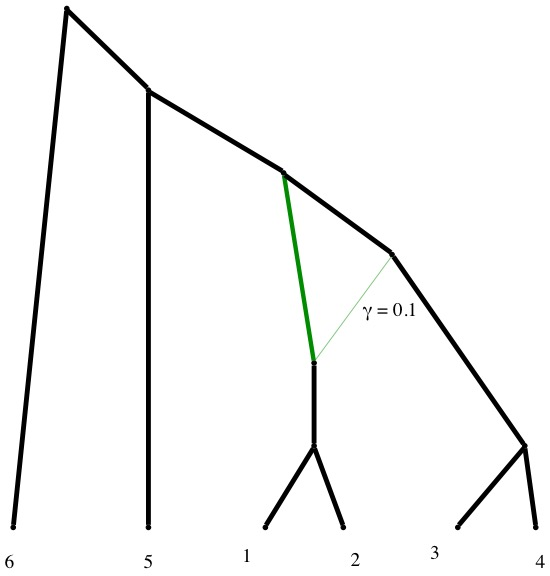
\includegraphics[scale=0.5]{figures/basicplot.pdf} \quad
    \caption{Basic plot using the \texttt{plotPhylonet} function. Note that if the gamma value for a hybrid edge is not explicitly defined, it will assume a default value of $0.1$.}
    \label{BasicPlot}
  \end{center}
\end{figure}

\noindent The user can combine any number of the following optional arguments to
customize the plot.
Given below are a few examples that exhibit the different visualization options available. \\

\noindent \textbf{Example 2:} For the sake of tidiness, we define the network  as its own variable, \texttt{net}.
In addition, we include the arguments \texttt{vert = false}, which plots the hierarchy horizontally,
\texttt{mainTree=true}, which only plots the underlying tree structure, and
\texttt{fontSize = 20.0}, which increases the label font size from 16.0 to 18.0. \\

\begin{lstlisting}
net = "(((((1,2))#H1,(#H1,(3,4))),5),6);"
PhyloNetworks.plotPhylonet(net, vert = false,
                           mainTree = true, fontSize = 20.0)
\end{lstlisting}

\begin{figure}[htbp]
  \begin{center}
    \includegraphics[scale=0.5]{figures/plot2.pdf} \quad
    \caption{Plot of the underlying tree structure, oriented horizontally, with a changed font size.}
    \label{BasicPlot}
  \end{center}
\end{figure}

% INCLUDE UNROOTED EXAMPLE

\subsubsection{Style Notes}
Although there are default argument values given by
\texttt{plotPhylonet}, they do not always result in the ideal plot for
a particular example.  Many of the included arguments were included
for the purpose of the user being able to adjust certain layout
parameters to best fit their own network.  In particular, there is
sometimes difficulty in neatly placing and orienting leaf labels and
gamma labels.  This is especially noticeable as the number of leaf
nodes becomes large or if the names associated with leaf nodes are
long.  We have included some tips for fixing common issues below.

\begin{itemize}
\item To avoid edges overlapping gamma labels, include the argument
  \texttt{edgeStyle = true}. This will allow the layout engine to
  include curved splines, which will avoid overlaps.
\item If leaf names are long, include the \texttt{vert = false}
  argument to set horizontal hierarchy.
\item Label overlap can also be finely altered by changing the
  \texttt{labelDistance} and \texttt{labelAngle} arguments.
\item Issues between in text readability can be fixed by adjusting the
  \texttt{fontSize}, \texttt{height}, or \texttt{width}.
\item Although the arguments \texttt{layoutStyle} and
  \texttt{edgeStyle} have been included, some of options available are
  not guaranteed to be ideal for certain network plots.
\end{itemize}

When plotting, a known issue can occur if Julia and GraphViz are not
linked. To test the GraphViz installation, see the following section:

\subsubsection{Example to test correct \texttt{GraphViz} installation}

The \texttt{GraphViz} package installs the program
\texttt{GraphViz}. To verify that the link between \texttt{Julia} and
\texttt{GraphViz} is working properly. Everything should be done
automatically, but it is worth testing.  Open \texttt{Julia} and type
\begin{lstlisting}
s=open("graph.dot","w")
write(s,"graph {
		a -- b;
		a -- c;
		b -- d;
		b -- e;
		c -- f;
		c -- g;
        f -- h;
        f -- i;
	}")
close(s)
PhyloNetworks.generalExport("graph.dot")
\end{lstlisting}
This will turn
\texttt{graph.dot} into a file called \texttt{genImage.svg} in the
working directory.

\noindent If this worked correctly, the console should display a series of prompts indicating its completion.
A file called \texttt{scratchimage.svg} should be located in your working directory.

\begin{center}
  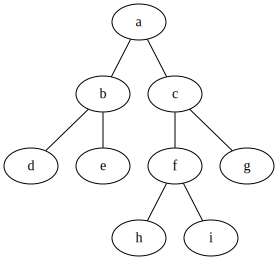
\includegraphics[width=3.0in]{figures/genImage.eps}
\end{center}
Plot of the underlying tree structure, oriented horizontally, with a changed font size.


\section{Version history}

\begin{itemize}
\item[\textbf{v0.0.2}]{Package fully implemented for Julia version v0.4 (does
    not support lower versions anymore). Faster way to extract quartets from
    input trees, and to extract a random sample of quartets without
    listing all quartets first; better functions to handle the case of
    multiple alleles (not 100\% robust, still testing in many
    scenarios)}
\end{itemize}



\bibliography{/Users/Clauberry/Documents/phylo/bibtex/Networks-prelim.bib}

\appendix
\section{Definition of Phylogenetic Network}

For the present work, we will use the following definition (but refer
to \citet{Huson2010} for other types of evolutionary networks).
A \textit{rooted phylogenetic network} for a set of taxa $X$ is a
connected directed acyclic graph with vertices $V=V_L \cup V_H \cup
V_T$, edges $E=E_H \cup E_T$ and a bijective leaf-labeling function
$f:V_L \rightarrow X$ with the following characteristics:
\begin{itemize}
\item The root $r$ has $\mathrm{indegree}(r)=0$ and $\mathrm{outdegree}(r)=2$.
\item{For any $v \in V_L$ (leaf), $indegree(v)=1$ and
    $outdegree(v)=0$.}
\item{For any $v \in V_T$ (tree node), $indegree(v)=1$ and $outdegree(v)=2$.}
\item{For any $v \in V_H$ (hybrid node), $indegree(v)=2$ and $outdegree(v)=1$.}
\item{A tree edge $e \in E_T$ is an edge whose child is a tree node.}
\item{A hybrid edge $e \in E_H$ is an edge whose child is a hybrid node.}
\end{itemize}
Thus, we are not allowing internal nodes with only two edges, nor
polytomies. We also do not allow a leaf to be hybrid node, and only 2
hybrid edges per hybrid node.

We assume that the hybridization cycles do not intersect, and these
networks are called \textit{level-1 networks} \citep{Huson2010}, which
have been shown to be identifiable \citep{Pardi2015,Solis-Lemus2015}.
These restrictions are enforced in the optimization, but not in the
read/write/plot/root functions. However, the only rule strictly
enforced for all functions is that a hybrid node cannot have more than
two hybrid edges pointing at it.

\end{document}
